\documentclass[a4paper]{article}
\usepackage[margin = 1 in]{geometry}
\usepackage{fancyhdr}
\usepackage{lastpage}
\usepackage{ctex}
\usepackage[utf8]{inputenc} % Required for inputting international characters
\usepackage[T1]{fontenc} % Output font encoding for international characters
\usepackage[sfdefault]{ClearSans} % Use the Clear Sans font (sans serif)
\usepackage{tocloft} 
\usepackage{makecell}%导入表格宏包
\usepackage{bmpsize}
\usepackage{graphicx}
\usepackage{epstopdf}
\usepackage{caption}
\usepackage{enumitem}
\usepackage{float}
\usepackage{multirow}
\usepackage{makecell}
\usepackage{wrapfig}
\usepackage{tcolorbox}
\usepackage[hidelinks]{hyperref}
\usepackage{xcolor}

\pagestyle{fancy}
\lhead{\textsl{\href{https://team23-22.bham.team}{\textcolor{blue}{Meeting Diary}}}}
\chead{}
\rhead{Page \thepage\ of \pageref{LastPage}}
\lfoot{}
\rfoot{}
\cfoot{}
\renewcommand{\headrulewidth}{0.4pt}
\renewcommand{\footrulewidth}{0pt}
\renewcommand{\cftsecleader}{\cftdotfill{\cftdotsep}}
\newcommand{\tabincell}[2]{\begin{tabular}{@{}#1@{}}#2\end{tabular}} %单元格内换行

\renewcommand*\contentsname{Table of Contents}

\begin{document}

%----------------------------------------------------------------------------------------
%	TITLE PAGE
%----------------------------------------------------------------------------------------

\begin{titlepage}
	
	\rule{\linewidth}{5pt}
	\raggedleft
	\fontsize{38pt}{50pt}\selectfont
    \textbf{\\Team Project\\}
    \fontsize{28pt}{60pt}\selectfont 
    for\\
    \fontsize{38pt}{60pt}\selectfont 
    \textbf{Meeting Diary\\}
	
	\vfill % Space between the title box and author information
	
	%------------------------------------------------
	%	Author name and information
	%------------------------------------------------
	
	\parbox[t]{0.93\textwidth}{ % Box to inset this section slightly
		\raggedleft % Right align the text
		\large % Increase the font size
		{\Large By Team 23-22}\\[4pt] % Extra space after name
		Bogdan-Marian Gheorghe\_2329324\_bxg125\\
		Chance Egbon\_2194210\_cee010\\
		Gilead Bempah\_2296232\_gxb035\\
		Matthew Goulding\_2330080\_mxg183\\
		Samuel Okasia\_2345883\_sxo183\\
		Smit Navinkumar\_2327596\_sxn197\\
		Zijun Li\_2272583\_zxl183\\
	}
	
\end{titlepage}

{\noindent\begin{tabular}{|p{0.2\linewidth}|p{0.75\linewidth}|} 
	\hline
 \multicolumn{2}{|l|}{\textbf{Week 9: Meeting 1}}\\
 \hline
 \textbf{Date} & 18-4-2023\\
 \hline
 \textbf{Time} & 14:20-14:40(UK Time Zone)\\
 \hline
 \textbf{Venue} & Room 222 CS Building\\
 \hline
 \multirow{3}*{\textbf{Attendees}} & Meeting Chair: Christian Vergara Marcillo \\
 ~ & Other Participants: Gilead Bempah, Matthew Goulding, Zijun Li\\
 ~ & through teams:  Smit Navinkumar\\
 \hline
 {\textbf{Discussions}} & During this meeting, the team focused on understanding the requirements for S3 as explained by the TA. In addition to discussing the expectations for S3, the TA also emphasized the importance of beginning preparations for M3. \\
 \hline
 \multirow{3}*{\textbf{Decisions Made}} & The team decided to diligently review and follow the guidelines provided by the TA for S3 to ensure all requirements are met in a timely and efficient manner.\\
 ~ & Members agreed to allocate time and resources for M3 preparations, recognizing the importance of planning ahead for the next phase.\\
 \hline
\end{tabular}}

{\noindent\begin{tabular}{|p{0.2\linewidth}|p{0.75\linewidth}|} 
	\hline
 \multicolumn{2}{|l|}{\textbf{Week 10: Meeting 1}}\\
 \hline
 \textbf{Date} & 25-4-2023\\
 \hline
 \textbf{Time} & 14:20-14:40(UK Time Zone)\\
 \hline
 \textbf{Venue} & Room 222 CS Building\\
 \hline
 \multirow{2}*{\textbf{Attendees}} & Meeting Chair: Christian Vergara Marcillo \\
 ~ & Other Participants: Gilead Bempah, Matthew Goulding, Zijun Li\\
 \hline
 {\textbf{Discussions}} & In this meeting, the team reviewed the completion status of each member's S3 section and discussed the feedback provided by the TA. Key points included the proper understanding of vertical slicing, which involves showcasing the frontend, backend, and database aspects of the project. The team discussed using JDL to demonstrate the entity framework, accessing the H2 database, and providing screenshots to illustrate the database section. Additionally, the importance of including GitLab commit links in the development section was addressed.\\
 \hline
 \multirow{3}*{\textbf{Decisions Made}} & The team decided to follow the TA's advice and ensure that the concept of vertical slicing is accurately represented in their project documentation and demonstration.\\
 ~ & Members agreed to utilize JDL for illustrating the entity framework, providing a clear and concise representation of the project structure.
 The team committed to accessing the H2 database and including relevant screenshots in their documentation to effectively showcase the database aspects of the application.\\
 ~ & To maintain transparency and traceability in the development process, the team decided to include GitLab commit links in the development section of their documentation, demonstrating the progress and contributions made by each member.\\
 \hline
\end{tabular}}

{\noindent\begin{tabular}{|p{0.2\linewidth}|p{0.75\linewidth}|} 
	\hline
 \multicolumn{2}{|l|}{\textbf{Week 11: Meeting 1}}\\
 \hline
 \textbf{Date} & 1-5-2023\\
 \hline
 \textbf{Time} & 16:00-21:00(UK Time Zone)\\
 \hline
 \textbf{Venue} & Room 245 CS Building\\
 \hline
 {\textbf{Attendees}} &  Gilead Bempah, Matthew Goulding, Zijun Li, Samuel Okasia, Smit Navinkumar, Bogdan-Marian Gheo-
 rghe\\
 \hline
 {\textbf{Discussions}} & During the meeting, the team reviewed the progress of each individual's feature implementation, assessing participation and completion status. Members also discussed the recent addition of the dark mode functionality, which required minor code modifications. The team shared their experiences and offered support to one another in order to achieve the best possible results.\\
 \hline
 \multirow{3}*{\textbf{Decisions Made}} & A decision was made to allocate time for addressing any necessary code modifications related to the dark mode implementation, in order to ensure a consistent user experience across both light and dark modes.\\
 ~ & The team committed to fostering a collaborative environment, where members can openly ask for assistance or provide support to others in completing their tasks.\\
 ~ & To keep everyone informed and maintain transparency, the team decided to hold regular progress check-ins, discussing any challenges faced and solutions implemented, and adjusting timelines if needed.\\
 \hline
\end{tabular}}

\begin{figure}
	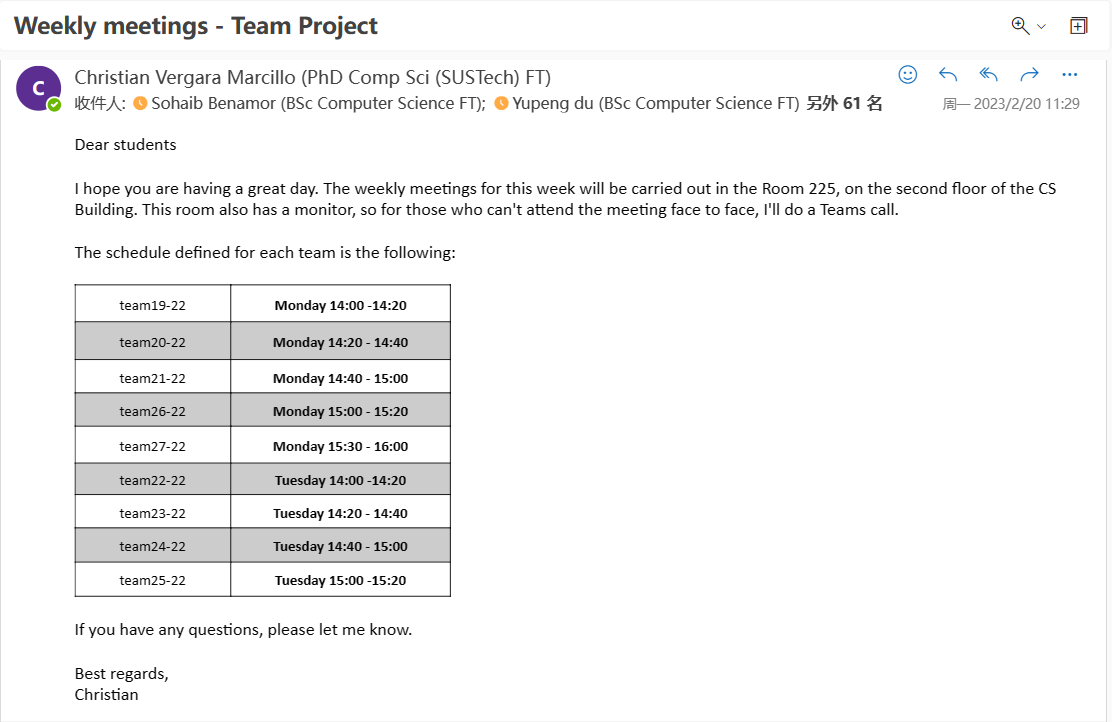
\includegraphics[width=\linewidth]{./image/meeting.png}
	\caption*{Evidence for weekly meeting}
\end{figure}

{\noindent\begin{tabular}{|p{0.2\linewidth}|p{0.75\linewidth}|} 
	\hline
 \multicolumn{2}{|l|}{\textbf{Week 11: Meeting 2}}\\
 \hline
 \textbf{Date} & 2-5-2023\\
 \hline
 \textbf{Time} & 14:20-14:40(UK Time Zone)\\
 \hline
 \textbf{Venue} & Room 222 CS Building\\
 \hline
 \multirow{2}*{\textbf{Attendees}} & Meeting Chair: Christian Vergara Marcillo \\
 ~ & Other Participants: Gilead Bempah, Matthew Goulding, Zijun Li, Samuel Okasia\\
 \hline
 \multirow{2}*{\textbf{Attendees}} & In person: Gilead Bempah, Matthew Goulding, Zijun Li, Samuel Okasia\\
 ~ & In discord: Smit Navinkumar, Chance Egbon\\
 \hline
 {\textbf{Discussions}} & During the meeting, the TA reviewed the complete web application and provided explanations and suggestions for the M3 requirements. The team members then demonstrated the application and its implemented features, ensuring a comprehensive understanding of the project's progress.\\
 \hline
 \multirow{3}*{\textbf{Decisions Made}} & For the demo video, the team decided that each feature must be thoroughly explained, with the allocated time for each section controlled within 1 minute\\
 ~ & The login interface was identified as an area that still requires optimization for better user experience.\\
 ~ & When showcasing the different features, the team agreed to emphasize their practicality and ease of use, highlighting how each feature contributes to effective time management for the user.\\
 \hline
\end{tabular}}

{\noindent\begin{tabular}{|p{0.2\linewidth}|p{0.75\linewidth}|} 
	\hline
 \multicolumn{2}{|l|}{\textbf{Week 11: Meeting 3}}\\
 \hline
 \textbf{Date} & 2-5-2023\\
 \hline
 \textbf{Time} & 14:30-(UK Time Zone)\\
 \hline
 \textbf{Venue} & Murray Learning Center\\
 \hline
 \multirow{2}*{\textbf{Attendees}} & In person: Gilead Bempah, Matthew Goulding, Zijun Li, Samuel Okasia\\
 ~ & In discord: Smit Navinkumar, Chance Egbon\\
 \hline
 {\textbf{Discussions}} & During the meeting, the team focused on consolidating individual contributions for the M3 requirements, discussing code optimization, and improving the user interface aesthetics. The team also engaged in a thorough examination of the codebase, sharing insights and identifying potential areas for further improvement, ensuring that the application is robust and efficient. \\
 \hline
 \multirow{2}*{\textbf{Decisions Made}} & The team agreed to conduct a comprehensive review of the application, with each member responsible for checking their respective contributions and verifying that all requirements have been met.\\
 ~ & The team decided to establish a clear plan for finalizing the application, including deadlines for completing tasks and a strategy for addressing any remaining issues discovered during the review process.\\
 \hline
\end{tabular}}

\end{document}